%La Fundamentación Teórica consiste en el planteamiento de:
% A. La perspectiva desde donde se desarrollará el estudio (modelo teórico, básico).
% B. Los elementos del tema que se consideran más significativos (variables con las cuales va a interactuar el investigador).
% C. Los instrumentos teóricos de análisis de los datos.

Para el desarrollo de este proyecto partimos a partir de la generación de señales artificiales que sustituirán a un sujeto de prueba real. Esto nos permitirá tener más señales con mayor variabilidad así como un mayor control del tipo de señal que queramos manejar. Para lograr esto partiremos de un modelo que aprenda los patrones de las señales de EEG y nos genere nuevos patrones con las mismas características.

\subsection{Redes Neuronales Recurrentes y LSTM}

Las Redes Neuronales Recurrentes (RNN) están diseñadas para procesar secuencias temporales, lo cual las hace ideales para generar señales EEG, que son dependientes del tiempo. Sin embargo, las RNN tradicionales presentan dificultades al aprender dependencias de largo plazo, debido al problema del desvanecimiento del gradiente. Para mitigar esta limitación, se han propuesto las celdas de Memoria a Largo y Corto Plazo (Long Short-Term Memory, LSTM), que incorporan puertas de entrada, olvido y salida, permitiendo retener información relevante a lo largo de la secuencia.

En el contexto de generación de señales, un modelo LSTM puede ser entrenado de manera autorregresiva para predecir la siguiente muestra de una señal a partir de una secuencia anterior, o bien, para reconstruir secuencias completas a partir de entradas parciales. El objetivo del entrenamiento consiste en minimizar la diferencia entre la señal original y la señal generada, usualmente mediante una función de pérdida como el error cuadrático medio (MSE).

\begin{equation}
\mathcal{L}_{\text{MSE}} = \frac{1}{n} \sum_{i=1}^{n} \left( y_i - \hat{y}_i \right)^2
\end{equation}

donde $y_i$ representa la muestra real y $\hat{y}_i$ la predicción del modelo.

\subsection{Autoencoders Variacionales (VAE)}

Los Autoencoders Variacionales (VAE) representan otra familia de modelos generativos ampliamente utilizados en el procesamiento de datos biomédicos. A diferencia de los autoencoders clásicos, los VAE aprenden una representación latente probabilística de los datos. En lugar de codificar cada entrada como un punto fijo en el espacio latente, el encoder estima una distribución (usualmente gaussiana) desde la cual se muestrean los vectores latentes.

Este enfoque permite generar nuevas señales al muestrear desde el espacio latente aprendido y decodificarlas en el dominio de la señal EEG. Formalmente, el VAE optimiza una pérdida compuesta por dos términos: la reconstrucción de la señal y la divergencia Kullback-Leibler (KL) entre la distribución latente aprendida y una distribución normal estándar:

\begin{equation}
\mathcal{L}_{\text{VAE}} = \mathbb{E}_{q(z|x)}[\log p(x|z)] - D_{KL}(q(z|x)\,\|\,p(z))
\end{equation}

donde $q(z|x)$ es la distribución aproximada del codificador, $p(z)$ es la distribución prior (usualmente $\mathcal{N}(0, I)$), y $p(x|z)$ es la distribución decodificada.

\subsection{Evaluación de la Calidad de Señales EEG Generadas}

Para evaluar nuestras señales usaremos métricas enfocadas en similitud estadística y fisiológica con las señales reales:

\begin{itemize}
    \item \textbf{Distribución espectral:} comparación de la densidad de potencia en diferentes bandas de frecuencia (\textit{delta, theta, alpha, beta, gamma}).
    \item \textbf{Medidas de complejidad:} tales como la entropía aproximada, entropía muestral, y dimensión fractal, que permiten evaluar la naturaleza no lineal de las señales EEG.
    \item \textbf{Coherencia intercanal:} análisis de la correlación funcional entre canales, útil para validar la preservación de patrones espacio-temporales.
    \item \textbf{Clasificabilidad:} uso de clasificadores entrenados en señales reales para evaluar si las señales generadas son indistinguibles a nivel de discriminación supervisada.
\end{itemize}


\subsection{Clasificación de Zonas Cerebrales a partir de Señales EEG}
Una vez que tengamos nuestras señales se avanzará a la siguiente etapa, enfocada en realizar un modelo que pueda predecir con eficacia la zona de activación cerebral, para lo cual abordaremos el problema como una tarea de clasificación multiclase supervisada en la que cada clase representa una región específica del cerebro.

Desde el punto de vista del modelado esta tarea cae dentro del denominado problema inverso, el cual consiste en estimar la fuente neuronal interna (ubicación y actividad) a partir de las señales de EEG medidas en el cuero cabelludo o en nuestro caso se utilizaran las señales generadas.

Es importante aclarar los dos problemas princiapales los cuales son:

\begin{itemize}
    \item Problema directo (forward problem): se refiere al cálculo de las señales EEG que se esperarían en los electrodos a partir de una distribución conocida de fuentes internas. Este proceso se resuelve utilizando modelos físicos del volumen conductor (por ejemplo, el modelo de cabeza), y se basa en las ecuaciones de Maxwell simplificadas bajo condiciones cuasiestáticas.

    \item Problema inverso (inverse problem): consiste en estimar las fuentes cerebrales responsables de las señales observadas. Debido a su naturaleza en la que no tiene una única solución ya que muchas configuraciones internas de fuentes neuronales pueden generar la misma señal en los electrodos del cuero cabelludo, ademas de que pos su sensibilidad al ruido pequeñas variaciones pueden causar grandes diferencias en la estimación de la fuente, se requiere técnicas de regularización, restricciones espaciales o modelos probabilísticos para obtener soluciones estables.
\end{itemize}

Para el caso del problema inverso se abordara por medio de tecnicas de aprendizaje profundo, donde nuestro modelo aprenderá una correspondencia entre patrones espacio-temporales de las señales de EEG así como sus fuentes. Ya que la naturaleza de estas señales son temporales multivariadas se empleara arquitecturas que nos permitan explotar estas caracteristicas espacio-temporales como redes neuronales convolucionales (CNN), LSTM o híbridos CNN-LSTM.

\subsection{Redes BiLSTM}

Las Redes Neuronales Recurrentes Bidireccionales (BiLSTM por sus siglas en ingles) son una extensión de las LSTM tradicionales que procesan la secuencia de manera bidireccional es decir hacia adelante y hacia atrás permitiendo al modelo tener un contexto completo de la señal en cada punto temporal.

El modelo BiLSTM puede tomar como entrada una secuencia de forma $(T, C)$, donde $T$ representa el número de pasos temporales y $C$ el número de canales. El modelo aprende representaciones internas que se combinan en una capa densa con activación \textit{softmax} para clasificar la señal según la zona cerebral correspondiente.

\subsubsection{Modelos CNN + LSTM}

Una arquitectura híbrida comúnmente utilizada para señales EEG combina redes convolucionales (CNN) con LSTM. Las CNN extraen características locales a través de convoluciones aplicadas en el dominio temporal o espacial, detectando patrones como oscilaciones o cambios abruptos. Estas representaciones extraídas se alimentan a una capa LSTM que modela la evolución temporal de dichas características.

La arquitectura general se puede resumir de la siguiente manera:

\begin{itemize}
    \item \textbf{Entrada:} matriz de forma $(T, C)$, con $T$ pasos temporales y $C$ canales.
    \item \textbf{Bloque CNN:} extracción de características espaciales o temporales.
    \item \textbf{Bloque LSTM:} modelado de dependencias a largo plazo.
    \item \textbf{Capa densa:} clasificación con activación \textit{softmax}.
\end{itemize}

Este tipo de arquitectura permite capturar tanto las relaciones entre electrodos (espaciales) como la evolución de la actividad neuronal en el tiempo (temporales), siendo altamente efectiva para tareas de identificación de zonas cerebrales.

\begin{figure}[H]
    \centering
    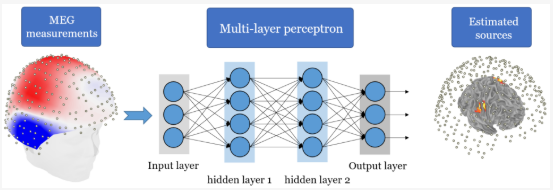
\includegraphics[scale=0.5]{figures/met/process.png}
    \caption{Ilustracion de la localizacion de fuentes MEG basado en modelo inverso\cite{Pantazis2021}}
    \label{fig:process}
\end{figure}

\subsubsection{Evaluación del Modelo}

La efectividad del modelo se evaluara utilizando métricas clásicas de clasificación como precisión, exactitud, sensibilidad, F1-score y matriz de confusión por clase (zona cerebral).

